%brent's poster layout :)

\documentclass[article,30pt,extrafontsizes]{memoir}

%utf-8 seems to be important
\usepackage[utf8]{inputenc}
\usepackage[T1]{fontenc}
\usepackage{palatino}
\usepackage{multicol}
\usepackage{graphicx}
\usepackage{blindtext}
\usepackage[svgnames,table]{xcolor}
\usepackage[framemethod=tikz]{mdframed}
\usepackage{color}
\usepackage{geometry}
\usepackage{adjmulticol}

%For kable extra package :)
\usepackage{booktabs}
\usepackage{longtable}
\usepackage{array}
\usepackage{multirow}
\usepackage{wrapfig}
\usepackage{float}
\usepackage{colortbl}
\usepackage{pdflscape}
\usepackage{tabu}
\usepackage{threeparttable}
\usepackage{threeparttablex}
\usepackage[normalem]{ulem}
\usepackage{makecell}


%For figure and table placement
\usepackage{float}
\floatplacement{figure}{H}
\floatplacement{table}{H}

%spacing between figure/ table and caption
\setlength{\abovecaptionskip}{0.4in}
\setlength{\belowcaptionskip}{0.2in}
\captionnamefont{\footnotesize\sffamily\bfseries}
\captiontitlefont{\footnotesize\sffamily}

%define column options
\setlength{\columnseprule}{1pt}
\def\columnseprulecolor{\color{red}}
\setsubsubsecheadstyle{\small\color{red}\textbf}% Set \section style
\setsecheadstyle{\small\color{red}}
\setsecnumformat{}
\def\sectionmark#1{\markboth{#1}{#1}}

%-----------------------------------------------------

\thispagestyle{empty}
\definecolor{light-gray}{gray}{0.9}

\usepackage[style=numeric,backend=biber]{biblatex}
\renewcommand*{\bibfont}{\tiny}

\bibliography{MyLibrary}
\author{Brent Thorne}
\title{Using \color{Red} \texttt{posterdown} \color{White} to generate
reproducible conference posters via RMarkdown \textgreater{} Knitr
\textgreater{} Markdown \textgreater{} Pandoc \textgreater{} Latex
\textgreater{} PDF workflow as well as long titles\ldots{}}
\counterwithout{section}{chapter}
\makechapterstyle{mydefault}{
\addtocounter{secnumdepth}{2}
\setsecheadstyle{\Large\color{red}\textbf}
\setsubsecheadstyle{\itshape}
\setsubsubsecheadstyle{\itshape}
}

\chapterstyle{mydefault}

\defbibheading{bibliography}[\bibname]{%
\section*{#1}%
\markboth{#1}{#1}}


\AtBeginDocument{%
  \renewcommand{\bibname}{References}
}


%define column spacing
\setlength\columnsep{1in}

\setlength\parindent{1em}
\setlength\parskip{1em}
\setlength\hangparas{0}

%spacing after section head title
\setaftersecskip{1in}
\setbeforesecskip{0.1in}
\setlength\textfloatsep{0.3in}
\setlength\floatsep{0.3in}
\setlength\intextsep{0.3in}

\setstocksize{38in}{45in}
\settrimmedsize{\stockheight}{\stockwidth}{*}
\settypeblocksize{38in}{45in}{*}
\setlrmargins{*}{*}{1}
\setulmarginsandblock{2.5cm}{*}{*}
\setmarginnotes{0em}{0cm}{0cm}
\setlength{\footskip}{0cm}
\setlength{\footnotesep}{0cm}
\setlength{\headheight}{0pt}
\setlength{\headsep}{0pt}
\setlength{\trimtop}{0pt}
\setlength{\trimedge}{0pt}
\setlength{\uppermargin}{0pt}
\checkandfixthelayout

\definecolor{myframecolour}{HTML}{00004d}

% see https://stackoverflow.com/a/47122900
\usepackage{color}
\usepackage{fancyvrb}
\newcommand{\VerbBar}{|}
\newcommand{\VERB}{\Verb[commandchars=\\\{\}]}
\DefineVerbatimEnvironment{Highlighting}{Verbatim}{commandchars=\\\{\}}
% Add ',fontsize=\small' for more characters per line
\usepackage{framed}
\definecolor{shadecolor}{RGB}{248,248,248}
\newenvironment{Shaded}{\begin{snugshade}}{\end{snugshade}}
\newcommand{\KeywordTok}[1]{\textcolor[rgb]{0.13,0.29,0.53}{\textbf{#1}}}
\newcommand{\DataTypeTok}[1]{\textcolor[rgb]{0.13,0.29,0.53}{#1}}
\newcommand{\DecValTok}[1]{\textcolor[rgb]{0.00,0.00,0.81}{#1}}
\newcommand{\BaseNTok}[1]{\textcolor[rgb]{0.00,0.00,0.81}{#1}}
\newcommand{\FloatTok}[1]{\textcolor[rgb]{0.00,0.00,0.81}{#1}}
\newcommand{\ConstantTok}[1]{\textcolor[rgb]{0.00,0.00,0.00}{#1}}
\newcommand{\CharTok}[1]{\textcolor[rgb]{0.31,0.60,0.02}{#1}}
\newcommand{\SpecialCharTok}[1]{\textcolor[rgb]{0.00,0.00,0.00}{#1}}
\newcommand{\StringTok}[1]{\textcolor[rgb]{0.31,0.60,0.02}{#1}}
\newcommand{\VerbatimStringTok}[1]{\textcolor[rgb]{0.31,0.60,0.02}{#1}}
\newcommand{\SpecialStringTok}[1]{\textcolor[rgb]{0.31,0.60,0.02}{#1}}
\newcommand{\ImportTok}[1]{#1}
\newcommand{\CommentTok}[1]{\textcolor[rgb]{0.56,0.35,0.01}{\textit{#1}}}
\newcommand{\DocumentationTok}[1]{\textcolor[rgb]{0.56,0.35,0.01}{\textbf{\textit{#1}}}}
\newcommand{\AnnotationTok}[1]{\textcolor[rgb]{0.56,0.35,0.01}{\textbf{\textit{#1}}}}
\newcommand{\CommentVarTok}[1]{\textcolor[rgb]{0.56,0.35,0.01}{\textbf{\textit{#1}}}}
\newcommand{\OtherTok}[1]{\textcolor[rgb]{0.56,0.35,0.01}{#1}}
\newcommand{\FunctionTok}[1]{\textcolor[rgb]{0.00,0.00,0.00}{#1}}
\newcommand{\VariableTok}[1]{\textcolor[rgb]{0.00,0.00,0.00}{#1}}
\newcommand{\ControlFlowTok}[1]{\textcolor[rgb]{0.13,0.29,0.53}{\textbf{#1}}}
\newcommand{\OperatorTok}[1]{\textcolor[rgb]{0.81,0.36,0.00}{\textbf{#1}}}
\newcommand{\BuiltInTok}[1]{#1}
\newcommand{\ExtensionTok}[1]{#1}
\newcommand{\PreprocessorTok}[1]{\textcolor[rgb]{0.56,0.35,0.01}{\textit{#1}}}
\newcommand{\AttributeTok}[1]{\textcolor[rgb]{0.77,0.63,0.00}{#1}}
\newcommand{\RegionMarkerTok}[1]{#1}
\newcommand{\InformationTok}[1]{\textcolor[rgb]{0.56,0.35,0.01}{\textbf{\textit{#1}}}}
\newcommand{\WarningTok}[1]{\textcolor[rgb]{0.56,0.35,0.01}{\textbf{\textit{#1}}}}
\newcommand{\AlertTok}[1]{\textcolor[rgb]{0.94,0.16,0.16}{#1}}
\newcommand{\ErrorTok}[1]{\textcolor[rgb]{0.64,0.00,0.00}{\textbf{#1}}}
\newcommand{\NormalTok}[1]{#1}

%begin the document
\begin{document}

\begin{mdframed}[backgroundcolor=myframecolour,linecolor=Red,topline=false,leftline=false,rightline=false,linewidth=2mm]

% group which adds title author and other infor
% Used instead of \maketitle for better spacing options
\begingroup
  \centering
  \color{White}
\vspace{1in}
  \Huge\textbf{Using \color{Red} \texttt{posterdown} \color{White} to generate
reproducible conference posters via RMarkdown \textgreater{} Knitr
\textgreater{} Markdown \textgreater{} Pandoc \textgreater{} Latex
\textgreater{} PDF workflow as well as long titles\ldots{}}\\[0.3in]
  \Large Brent Thorne \par
\vspace{1.2in}
% end title section -------------------
  \endgroup
\end{mdframed}

% Brgin body of poster
\color{black}
\begin{adjmulticols*}{3}{10mm}{10mm}
\normalsize{
\section{Introduction}\label{introduction}

Welcome to \texttt{posterdown} ! This is my attempt to provide a
semi-smooth workflow for those who wish to take their \texttt{RMarkdown}
skills to the conference world. Many creature comforts frim
\texttt{RMarkdown} are available in this package such as
\texttt{Markdown} section notation, figure captioning, and even
citations like this one \autocite{holden_identifying_2012} The rest of
this example poster will show how you can insert typical conference
poster features into your own document.

\section{Study Site}\label{study-site}

Here is a map made to show the study site using \texttt{ggplot2},
\texttt{ggspatial}, and \texttt{sf}. Lorem ipsum dolor sit amet,
\autocite{middleton_geological_nodate} consectetur adipiscing elit, sed
do eiusmod tempor incididunt ut labore et dolore magna aliqua. Phasellus
vestibulum lorem sed risus ultricies tristique nulla. Mauris vitae
ultricies leo integer malesuada nunc vel risus commodo. Suspendisse
potenti nullam ac tortor vitae. Enim nunc faucibus a pellentesque sit
amet porttitor eget. \vspace{15mm}

\begin{figure}

{\centering 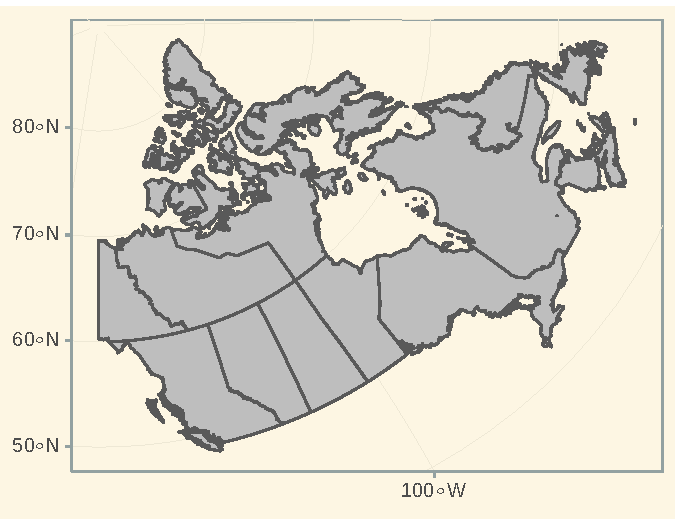
\includegraphics[width=0.8\linewidth]{skeleton_files/figure-latex/unnamed-chunk-2-1} 

}

\caption{This is a map of Canada, projected using the NAD 83 UTM Zone 7 Datum.}\label{fig:unnamed-chunk-2}
\end{figure}

\section{Objectives}\label{objectives}

\large

\begin{enumerate}
\def\labelenumi{\arabic{enumi}.}
\tightlist
\item
  Easy to use reproducible poster design.
\item
  Integration with \texttt{RMarkdown}.
\item
  Easy transition from \texttt{posterndown} to \texttt{thesisdown} or
  \texttt{rticles}
\end{enumerate}

\small

\section{Methods}\label{methods}

This package uses the same workflow approach as the \texttt{RMarkdown}
you know and love. Basically it goes from RMarkdown \textgreater{} Knitr
\textgreater{} Markdown \textgreater{} Pandoc \textgreater{} Latex
\textgreater{} PDF

\section{Results}\label{results}

\rowcolors{2}{gray!6}{white}

\begin{table}

\caption{\label{tab:unnamed-chunk-3}Hopefully this works without much of a headache!}
\centering
\begin{tabular}[t]{ccccc}
\hiderowcolors
\toprule
Sepal.Length & Sepal.Width & Petal.Length & Petal.Width & Species\\
\midrule
\showrowcolors
5.1 & 3.5 & 1.4 & 0.2 & setosa\\
4.9 & 3.0 & 1.4 & 0.2 & setosa\\
4.7 & 3.2 & 1.3 & 0.2 & setosa\\
4.6 & 3.1 & 1.5 & 0.2 & setosa\\
\bottomrule
\end{tabular}
\end{table}

\rowcolors{2}{white}{white}

\begin{Shaded}
\begin{Highlighting}[]
\CommentTok{# Here is some code for people}
\CommentTok{# to look at and be in awe of!!!!}
\KeywordTok{library}\NormalTok{(ggplot2)}
\KeywordTok{library}\NormalTok{(ggthemes)}

\KeywordTok{ggplot}\NormalTok{(}\DataTypeTok{data=}\NormalTok{iris,}
       \KeywordTok{aes}\NormalTok{(}\DataTypeTok{x =}\NormalTok{ Sepal.Width,}
           \DataTypeTok{y =}\NormalTok{ Sepal.Length,}
           \DataTypeTok{colour =}\NormalTok{ Species)) }\OperatorTok{+}
\StringTok{  }\KeywordTok{geom_point}\NormalTok{() }\OperatorTok{+}
\StringTok{  }\KeywordTok{theme_stata}\NormalTok{() }\OperatorTok{+}
\StringTok{  }\OtherTok{NULL}
\end{Highlighting}
\end{Shaded}

\begin{figure}

{\centering 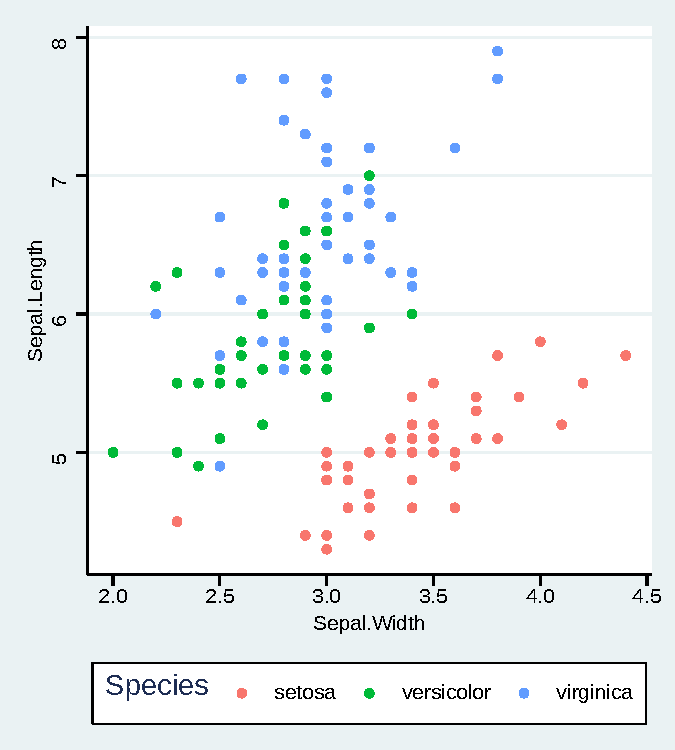
\includegraphics[width=0.8\linewidth]{skeleton_files/figure-latex/unnamed-chunk-4-1} 

}

\caption{Another figure showing how base R plots might look on this poster!}\label{fig:unnamed-chunk-4}
\end{figure}

\begin{figure}

{\centering 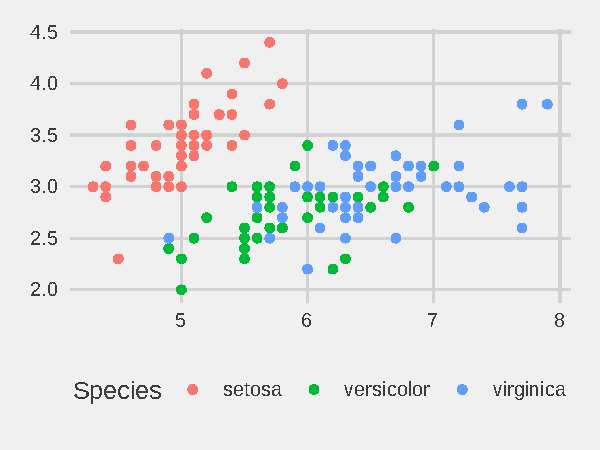
\includegraphics[width=0.75\linewidth]{skeleton_files/figure-latex/unnamed-chunk-5-1} 

}

\caption{A typical plot using ggplot.}\label{fig:unnamed-chunk-5}
\end{figure}

\section{Next Steps}\label{next-steps}

Pellentesque habitant morbi tristique senectus et netus. Magnis dis
parturient montes nascetur ridiculus mus mauris vitae ultricies. Nibh
nisl condimentum id venenatis. Lorem ipsum dolor sit amet consectetur
adipiscing elit duis. Eget aliquet nibh praesent tristique magna sit
amet purus. Orci phasellus egestas tellus rutrum. Mauris cursus mattis
molestie a. Amet cursus sit amet dictum sit. Tellus id interdum velit
laoreet. Tortor at risus viverra adipiscing. Ullamcorper malesuada proin
libero nunc. Elit ullamcorper dignissim cras tincidunt lobortis feugiat
vivamus. Eget dolor morbi non arcu risus quis. Pulvinar pellentesque
habitant morbi tristique senectus.

\small
\printbibliography
}
\end{adjmulticols*}
%end the poster
\end{document}
